\documentclass[a4 paper]{article}
%\usepackage{minted}           %embedding code
\usepackage{amsmath, amsthm, amsfonts} %always use amsmath for symbols, amsthm for theorems 
\usepackage{graphicx}  % for pictures
%\usepackage{lipsum}  % for test text
\usepackage{multicol}    % for multicollumn text
\usepackage[bottom=2.5cm]{geometry}   %to set the margins to your liking
\usepackage[skip = 10pt, indent = 30pt]{parskip}      %to set the distance between paragraphs
\usepackage{tcolorbox}           %for literal color boxes
%\usepackage{witharrows}             % understandable, arrows for equations
\usepackage{tikz}                   %drawings and diagrams
\usetikzlibrary{positioning}        %tikz library for positioning (of nodes?)
\usepackage{pgfplots}               %plotting and graphs
\pgfplotsset{compat=1.18, width = 10cm}
\usepackage{hyperref}
\hypersetup{colorlinks = true, linkcolor = black, urlcolor = blue}
%\usepackage{fancyvrb}           % fancy formatting of verbatim
%\usepackage{fancyhdr, lastpage}
%\pagestyle{fancy} 
%\lhead{Relat\'orio experimento 4}
%\rhead{FisExpI}
%\cfoot{Página \thepage \ de \pageref{LastPage}}
%\usepackage[Bjornstrup]{fncychap} %Sonny, Glenn, Lenny, Conny, Rejne, Bjarne, Bjornstrup
%\usepackage{xcolor}      %color text
%\usepackage{siunitx}    %for SI units
\usepackage{setspace}
\onehalfspacing
\usepackage{cleveref}
\usepackage[brazil]{babel}
\usepackage{caption}
\usepackage{subcaption}
\usepackage{pdfpages}
\usepackage{booktabs}
\usepackage{multirow}
\usepackage{textcomp}
\usepackage{amssymb}
\usepackage[document]{ragged2e}
\usepackage{bm}
\usepackage{empheq}




%\setlength{\hoffset}{-2cm}
%\setlength{\voffset}{1.5cm}                     %control your margins however you want!
%\setlength{\marginparwidth}{2cm}
%\setlength{\oddsidemargin}{0cm}

%\newtheorem{theorem}{Theorem}[section]               %how you call it and how you display it
%\newtheorem{corollary}{Corollary}[theorem]


\newcommand{\parag}{\hspace{30pt}}
%\newcommand{\pd}[2]{\frac{\partial#1}{\partial#2}}


\begin{document}


\justifying
\begin{center}{\large Laboratório de Circuitos Elétricos - 02/2024 - Turma 05}\\
{\large \textbf{Experimento 6}}\\ 
12/12/2024
\end{center}

\vspace{500pt}
 \noindent\textbf{Grupo 5:}\\
 Yuri Shumyatsky - 231012826\\
Vinicius de Melo Moraes - 231036274\\



\vspace{30pt}
\newpage

\section{Introdução}
\parag O estudo da potência em regime permanente senoidal é fundamental para a compreensão do comportamento de circuitos elétricos alimentados por sinais alternados (AC). Nesse regime, as grandezas elétricas, como corrente e tensão, assumem comportamentos senoidais que podem apresentar defasagem entre si devido à presença de elementos resistivos, indutivos e capacitivos. A análise da potência envolve conceitos como o fator de potencia, este que determina a proporção de potencia ativa e reativa, as quais são essenciais para o entendimento e o projeto de sistemas elétricos eficientes.



\vspace{5cm}
\section{Materiais}


	\begin{itemize}
	\item National Instruments Elvis II
	\item 1 capacitor de 100n$F$
	\item 2 resistores de 47$\Omega$
	\item 1 indutor de 1mH
	\end{itemize}

\newpage

\section{Procedimentos}
\parag Como usual, os componentes têm suas grandezas medidas para efeito de comparação. Os resultados são adicionados à Tabela 1.

\vspace{5pt}
\begin{table}[h]
\centering
\begin{tabular}{|c|c|c|c|}
\hline
\textbf{Grandeza} & \textbf{Valor nominal} & \textbf{Valor medido} & \textbf{Erro (\%) }\\\hline
R & 47$\Omega$ & 47.359$\Omega$ & 0.76 \\\hline 
L & 1mH & 0.863mH & 13.70 \\\hline 
C & 100nF & 107.500nF & 7.50 \\\hline 
\end{tabular}
\caption*{Tabela 1: Valores dos componentes}
\end{table}

Em seguida, é montado o circuito da Figura 1 e liga-se o gerador de funções do Elvis para obter uma onda senoidal com 2$V_{pp}$ e frequência de 14kHz.

\begin{table}[h]
\centering
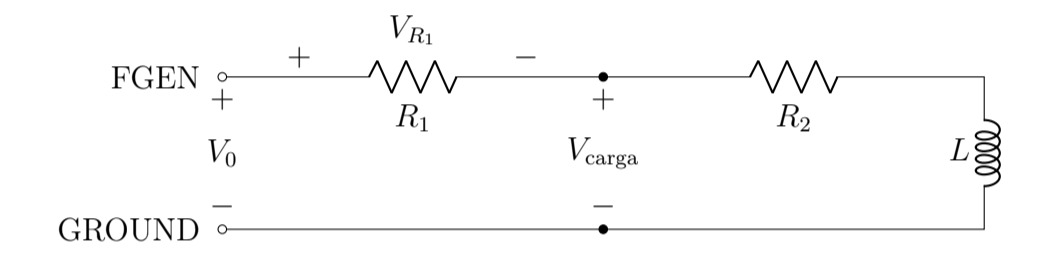
\includegraphics[scale=0.5]{figuras/figura1}
\end{table}

\begin{center}
Figura 1: Circuito sem capacitor
\end{center}

Fazendo análise nodal nesse circuito, são encontradas $V_0$ e $V_{carga}$, que serão usadas para encontrar $V_{R_1}$. 

\[\frac{V_{carga}-V_0}{47}+\frac{V_{carga}-V_2}{47}=0\]
\[\frac{V_2-0}{j14}-\frac{(V_{carga}-V_2)}{47}=0\]
\[\frac{V_0-1}{50}-\frac{(V_{carga}-V_0)}{47}=0\]


De onde obtém-se o seguinte sistema:

\begin{equation*}
\left\{
\begin{aligned}
2V_{carga}-V_0-V_2=0\\
-\frac{V_{carga}}{47} + \frac{V_0}{97} = \frac{1}{50}\\
-\frac{V_{carga}}{47} + V_2\left(-\frac{1}{47}-j\frac{1}{14}\right)=0\\
\end{aligned}\right.
\end{equation*}

\newpage
De onde obtemos os resultados 
\[V_0 = 0,63930+j0,02704=0,640\angle 2,42\text{\textdegree}\]
\[V_{carga}=0,30024+j0,05245=0,305\angle 9,91\text{\textdegree}\]
\[V_2=-0,038820+j0,077870=0,087\angle -63,50\text{\textdegree}\]

Com $V_0$ e $V_{carga}$ podemos encontrar $V_{R_1}=V_0-V_{carga}$\\
Portanto $V_{R_1}=0,33906-j0,02541=0,340\angle-4,29\text{\textdegree}$ 

Para senoides, o valor eficaz é simplesmente sua amplitude dividida por $\sqrt{2}$. Portanto, esses valores são calculados e dispostos na Tabela 2.

Com esses valores já pode ser montado o Gráfico 1, em que a senoide vermelha representa $V_0$ e a azul $V_{carga}$.

\vspace{3cm}
\begin{table}[h]
\centering
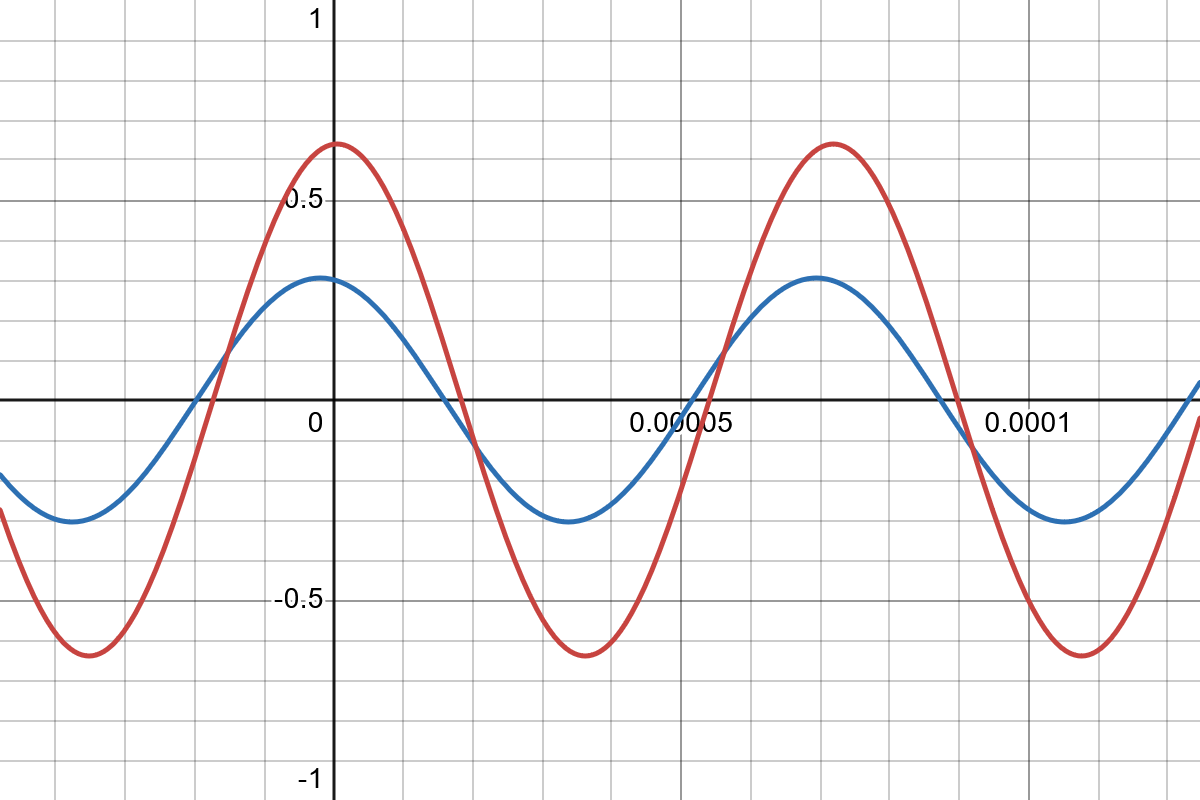
\includegraphics[scale=0.25]{rgadicoas/grafico1}
\end{table}

\begin{center}
Gráfico 1: Circuito sem capacitor (teórico)
\end{center}

\newpage


Para obter o fator de potência, usa-se a seguinte fórmula:

\[fp = \frac{|V_0|^2-|V_{R_1}|^2-|V_{carga}|^2}{2|V_{R_1}||V_{carga}|}\]

que é consequência do triângulo de potência, em que o fator de potência é o ângulo $\theta_v-\theta_i$


\vspace{2cm}
\begin{center}
\begin{tikzpicture}
\draw (0,0)--(4,3)--(4,0)--(0,0);
\draw node at (2,2) {\textbf{S}};
\draw node at (2,-0.7) {\textbf{P}};
\draw node at (4.5,1.5) {\textbf{Q}};
\draw (1,0) arc (0:38:1cm);
\draw node at (1.5,0.4) {$\theta_v-\theta_i$}; 
\end{tikzpicture}
\end{center}

\begin{center}
Figura 2: Triângulo de potência
\end{center}
\vspace{2cm}

Como $fp=cos(\theta_v-\theta_i)=\frac{P}{S}$ e sabendo que $V_0=V_{R_1}+V_{carga}$, \\temos que $(V_0)^2=(V_{R_1}+V_{carga})^2$
\[\implies|V_0|^2=|V_{R_1}|^2 + |V_{carga}|^2+2|V_{R_1}||V_{carga}|cos(\theta)\]
Isolando $cos(\theta)$ temos 
\[fp = cos(\theta)= \frac{|V_0|^2-|V_{R_1}|^2-|V_{carga}|^2}{2|V_{R_1}||V_{carga}|}\]

Portanto, usando os valores encontrados anteriormente, obtemos o valor de $fp$ para o circuito e eles são dispostos na Tabela 2.

Usando o osciloscópio do Elvis, são medidas as tensões $V_0$ e $V_{carga}$, obtidas no Gráfico 2. Esses valores são usados para obter $V_{R_1}$ e são encontrados na Tabela 2. 

\newpage

\begin{table}[h]
\centering
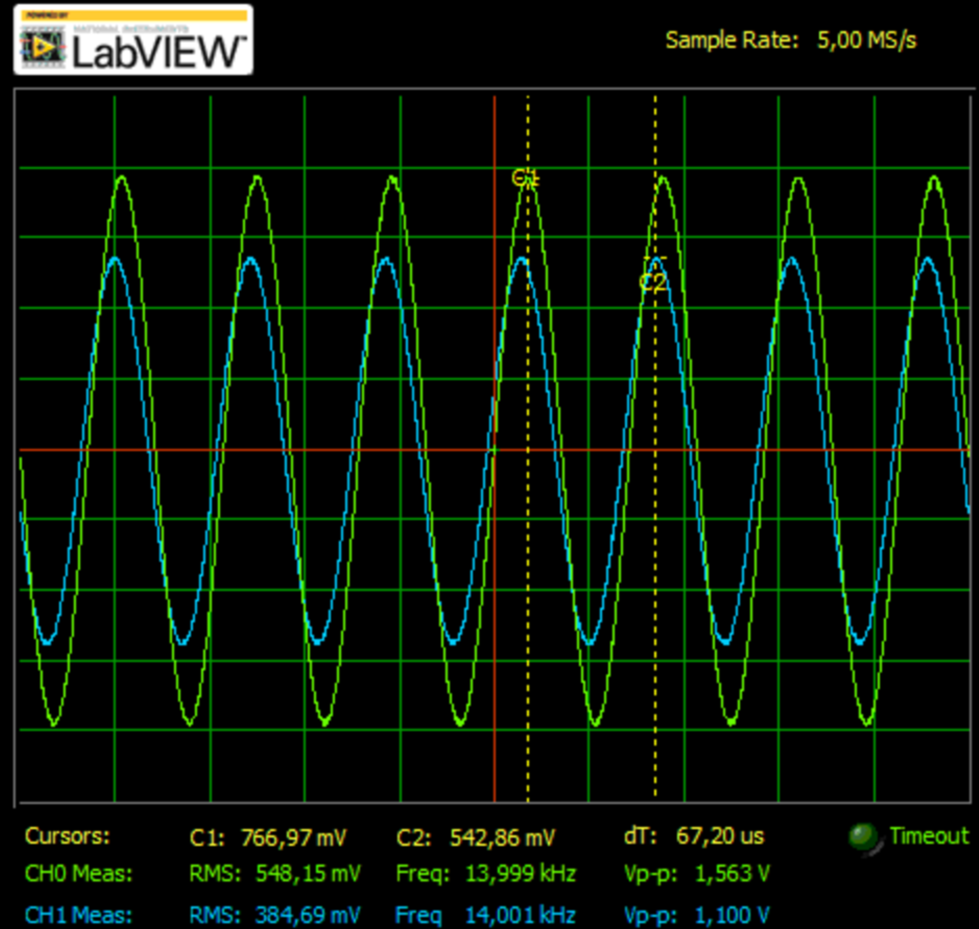
\includegraphics[scale=0.3575]{rgadicoas/rgadicoa1}
\end{table}

\begin{center}
Gráfico 2: Circuito sem capacitor
\end{center}

Assim, pode-se observar que experimentalmente os valores são $V_{0RMS}=0,553\angle0\text{\textdegree}$ e $V_{cargaRMS}=0,389\angle21,31\text{\textdegree},$ simplesmente como antes dividindo a amplitude por $\sqrt{2}$ e a fase é encontrada facilmente convertendo o dt de 4,22$\mu s$ para graus, usando a frequência de 14000Hz.

De forma análoga ao anterior, encontra-se $V_{R_1}=V_0-V_{carga}$ e seu valor RMS é simplesmente dividir esse valor por $\sqrt{2}$.

\vspace{1cm}
\vspace{5pt}
\begin{table}[h]
\centering
\begin{tabular}{|c|c|c|c|c|}
\hline
\textbf{Frequência (kHz)} & \textbf{Grandeza} & \textbf{Valor nominal} & \textbf{Valor medido} & \textbf{Erro (\%) }\\\hline
10   & $|V_0|$ & 1.57V & 1.55V & 1.27 \\\hline
10   & $|V_1|$ & 2.33V & 1.81V & 22.31 \\\hline
10   & $20log_{10}(|V_1|/|V_0|)$ & 3.434 & 1.347 & 60.77 \\\hline
10   & Fase de $V_1$ em relação a $V_0$ & -26.01\textdegree & -43.20\textdegree & 66.09 \\\hline
12.5 & $|V_0|$ & 1.25V & 1.38V & 10.40 \\\hline
12.5 & $|V_1|$ & 2.35V & 1.63V & 30.64 \\\hline
12.5 & $20log_{10}(|V_1|/|V_0|)$ & 5.481 & 1.446 & 73.62 \\\hline
12.5 & Fase de $V_1$ em relação a $V_0$ & -43.93\textdegree & -57.24\textdegree & 30.30 \\\hline
15.5 & $|V_0|$ & 0.97V & 1.34V & 38.14 \\\hline
15.5 & $|V_1|$ & 2.11V & 1.46V & 30.81 \\\hline
15.5 & $20log_{10}(|V_1|/|V_0|)$ & 6.733 & 0.745 & 88.94 \\\hline
15.5 & Fase de $V_1$ em relação a $V_0$ & -83.58\textdegree & -71.45\textdegree & 14.51 \\\hline
19.3 & $|V_0|$ & 1.17V & 1.34V & 14.53 \\\hline
19.3 & $|V_1|$ & 1.58V & 1.20V & 24.05 \\\hline
19.3 & $20log_{10}(|V_1|/|V_0|)$ & 2.626 & -0.958 & 136.48 \\\hline
19.3 & Fase de $V_1$ em relação a $V_0$ & -129.54\textdegree & -94.48\textdegree & 27.06 \\\hline
24.1 & $|V_0|$ & 1.51V & 1.47V & 2.65 \\\hline
24.1 & $|V_1|$ & 1.02V & 0.89V & 12.75 \\\hline
24.1 & $20log_{10}(|V_1|/|V_0|)$ & -3.381 & -4.359 & 28.93 \\\hline
24.1 & Fase de $V_1$ em relação a $V_0$ & -151.17\textdegree & -121.47\textdegree & 19.65 \\\hline
30   & $|V_0|$ & 1.72V & 1.64V & 4.65 \\\hline
30   & $|V_1|$ & 0.64V & 0.63V & 1.56 \\\hline
30   & $20log_{10}(|V_1|/|V_0|)$ & -8.635 & -4.155 & 51.88 \\\hline
30   & Fase de $V_1$ em relação a $V_0$ & -160.86\textdegree & -129.49\textdegree & 19.51 \\\hline
\end{tabular}
\caption*{Tabela 2: Valores referentes ao circuito 1}
\end{table}

\vspace{1cm}
Em seguida, é introduzido o capacitor no circuito, como indicado na Figura 3. 

\vspace{3cm}
\begin{table}[h]
\centering
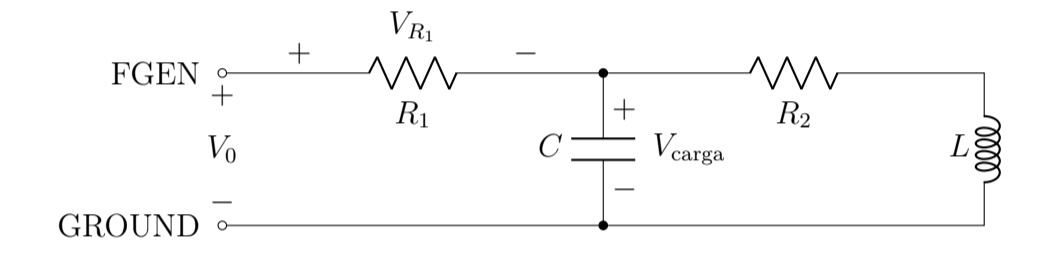
\includegraphics[scale=0.5]{figuras/figura2}
\end{table}

\begin{center}
Figura 3: Circuito com capacitor 
\end{center}

Usando análise de malhas para descobrir $V_0$ e $V_{carga}$ obtemos o seguinte sistema:

\begin{equation*}
\left\{
\begin{aligned}
50\textbf{I}_1+47\textbf{I}_2-j(\textbf{I}_1-\textbf{I}_2)=1\\
-\frac{j}{1,4\cdot10^{-3}}(\textbf{I}_2-\textbf{I}_1)+(47+j14)\textbf{I}_2=0
\end{aligned}\right.
\end{equation*}

Resolvendo esse sistema, obtemos os valores para as correntes:

\[\textbf{I}_1=0,0068254-j0,0005160\]
\[\textbf{I}_2=0,0068955-j0,009891\]


Com esses valores, usamos as relações $1-V_0=50\textbf{I}_1$ e $V_{carga}=(\textbf{I}_1-\textbf{I}_2)\cdot\frac{-j}{14\cdot10^{-3}}$ para encontrar $V_0=0,659+j0,0258=0,659\angle2,24\text{\textdegree}$ e $V_{carga}=0,338+j0,050=0,342\angle8,41\text{\textdegree}$.

De forma análoga ao feito anterior, $V_{R_1}=V_0-V_{carga}=0,321-j0,024=0,322\angle-4,28\text{\textdegree}$. As amplitudes, fases e valores RMS são todos calculadas exatamente da mesma forma que antes e dispostas na Tabela 3.

Além disso, $fp=0,970$, usando a fórmula disposta anteriormente.

Com esses valores, monta-se o Gráfico 3, em que a senoide azul representa $V_0$ e a vermelha representa $V_{carga}$.

\newpage
\vspace{3cm}
\begin{table}[h]
\centering
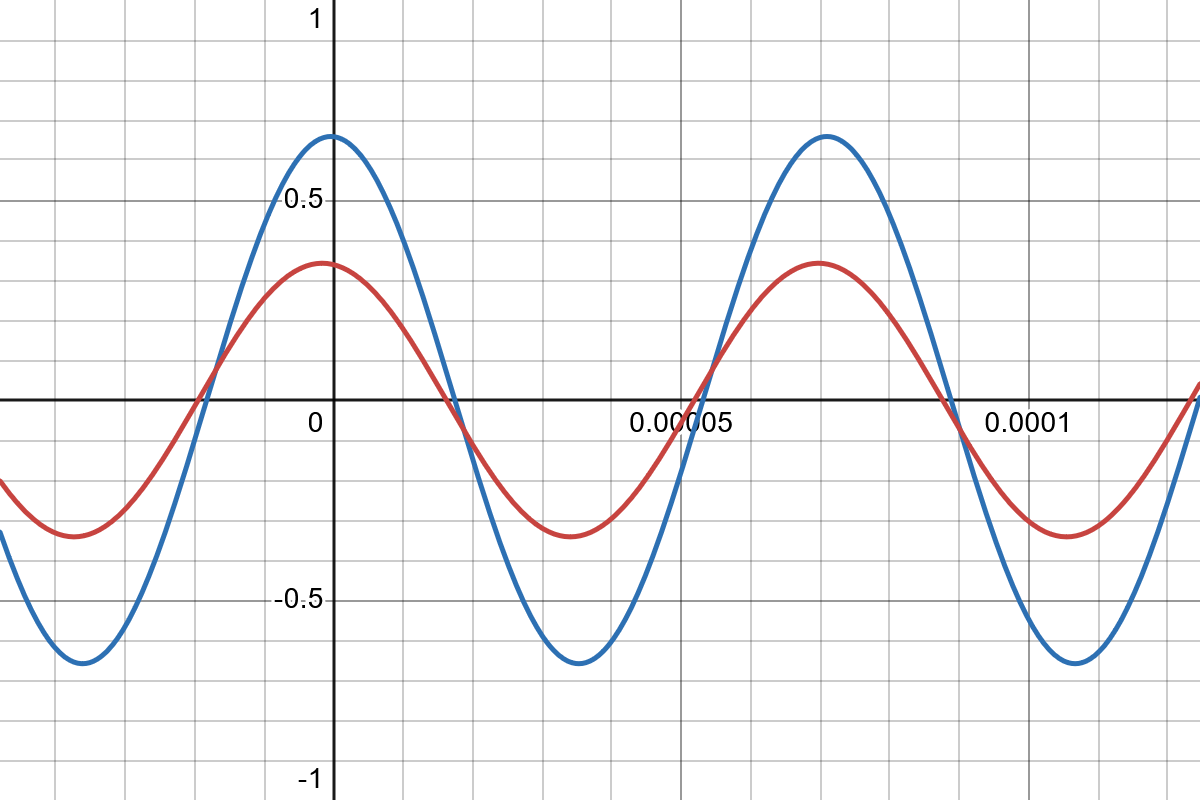
\includegraphics[scale=0.25]{rgadicoas/grafico2}
\end{table}

\begin{center}
Gráfico 3: Circuito com capacitor (teórico)
\end{center}

Nota-se que a presença do capacitor "desfaz" o adiantamento proporcionado pelo indutor no primeiro circuito.

Para a parte prática, repete-se o procedimento, gerando o Gráfico 4.


\begin{table}[h]
\centering
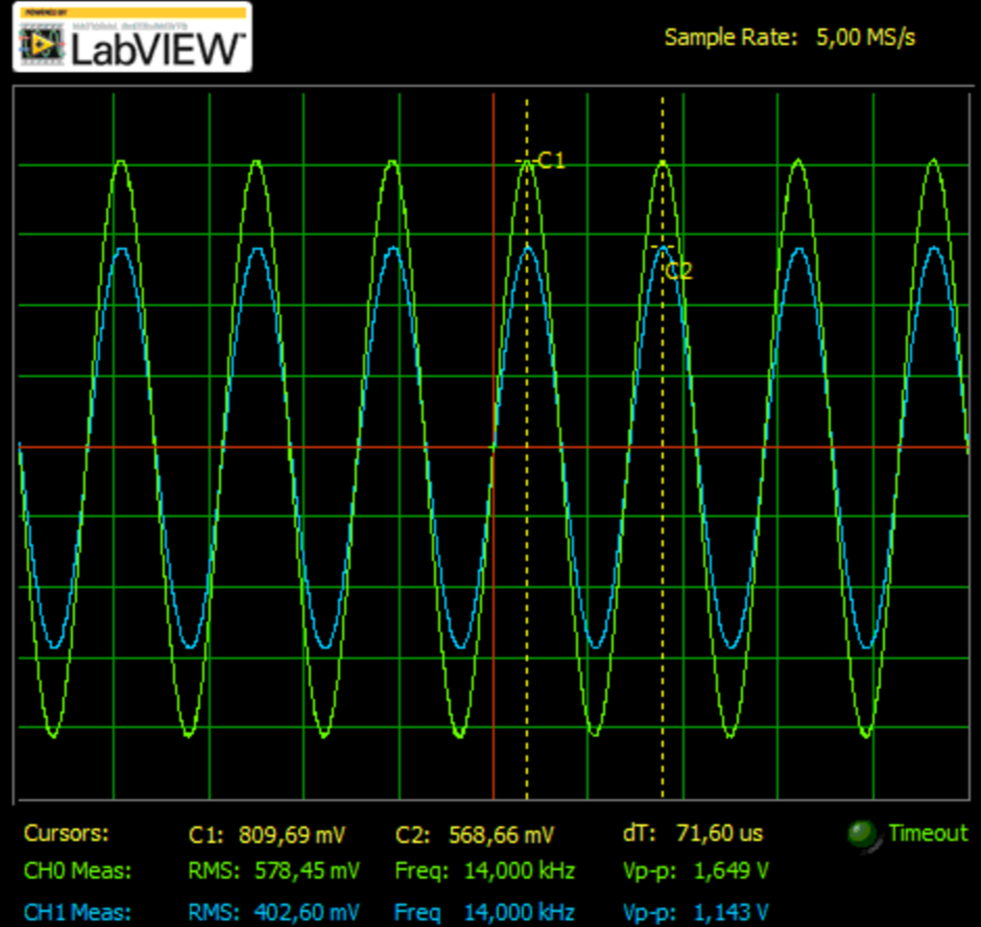
\includegraphics[scale=0.25]{rgadicoas/rgadicoa2}
\end{table}

\begin{center}
Gráfico 4: Circuito com capacitor 
\end{center}

A partir do Gráfico 4 são extraídas as informações relevantes, como:


\begin{minipage}{0.4\textwidth}
\begin{align*}
V_{carga}&=0,572\angle-0,864\text{\textdegree}\\
V_0&=0,825\angle0\text{\textdegree}\\
V_{R_1}&=0,253\angle1,95\text{\textdegree}
\end{align*}
\end{minipage}
\begin{minipage}{0.4\textwidth}
\begin{align*}
V_{cargaRMS}=0,404\\
V_{0RMS}=0,583\\
V_{R_1RMS}=0,179
\end{align*}
\end{minipage}

\newpage
\vspace{5pt}
\begin{table}[h]
\centering
\begin{tabular}{|c|c|c|c|}
\hline
\textbf{Grandeza} & \textbf{Valor nominal} & \textbf{Valor medido} & \textbf{Erro (\%) }\\\hline
$v_0$ & 1V & 1.006V & 0.6 \\\hline
$v_1$ & 3.2V & 2.315V & 27.66 \\\hline
$v_-$ & 1V & 1.007V & 0.7 \\\hline
$V^+$ & 10V & 9.994V & 0.6 \\\hline
$V^-$ & -10V & -10.005V & 0.5 \\\hline
$i_+$ & 0A & 0.195A & - \\\hline
$i_-$ & 0A & 4.158mA & - \\\hline
\end{tabular}
\caption*{Tabela 1: Valores dos componentes}
\end{table}



\vspace{3cm}\section{Conclusão}
\parag O experimento realizado permitiu analisar o comportamento da potência em circuitos elétricos no regime permanente senoidal. Observou-se que a presença de elementos resistivos, indutivos e capacitivos provoca a defasagem entre corrente e tensão, influenciando diretamente o fator de potência. Esse parâmetro se mostrou essencial para determinar a relação entre a potência ativa, responsável pelo trabalho útil no circuito, e a potência reativa, associada ao armazenamento de energia nos componentes indutivos e capacitivos.

Os resultados obtidos demonstraram a importância de otimizar o fator de potência para garantir maior eficiência nos sistemas elétricos, reduzindo perdas e melhorando o desempenho geral dos circuitos. Dessa forma, o experimento reforçou a relevância do estudo da potência no regime senoidal e a aplicação prática dos conceitos teóricos em projetos e análises de sistemas elétricos.


\section{Bibliografia}

\begin{itemize}
\item HALLIDAY, D.; RESNICK, R.; WALKER, J. Fundamentos de Física. 10. ed. v. 3. Rio de Janeiro: LTC, 2016.
\end{itemize}

\end{document}